%\begin{figure}[htb]
%\begin{center}
%  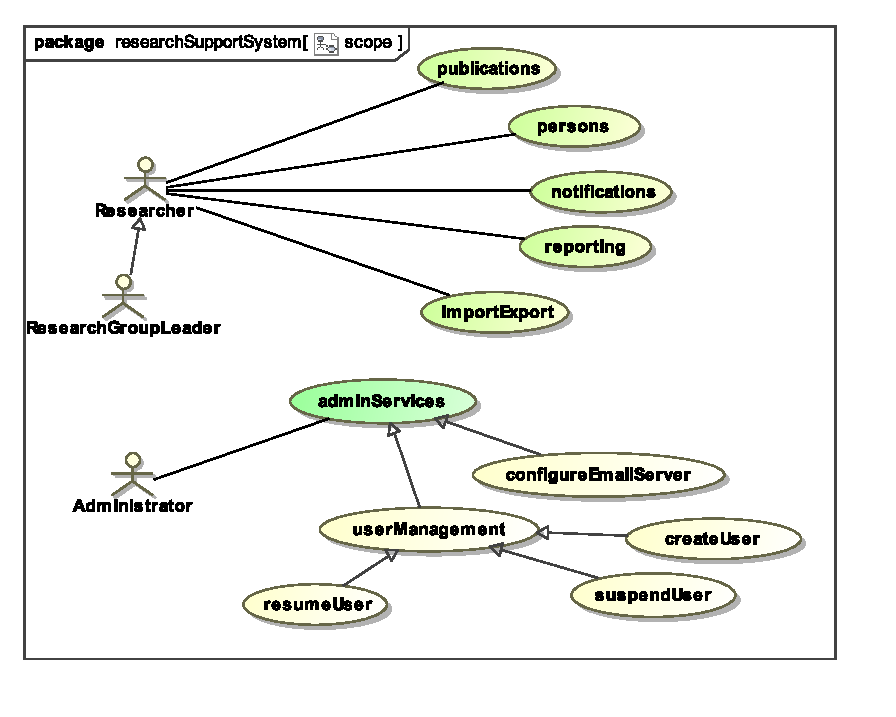
\includegraphics[width=0.9\textwidth,height=0.5\textheight,keepaspectratio=true]{scope}
%\end{center}
%\caption{The scope of Pinoccio. \label{fig:scope}}
%\end{figure}

Pinocchio consist of the following Modules.  
\begin{description}
\item[User Module] \hfill \\ for user authentication and maintenance of user information.
\item[Survey Module] \hfill \\  for maintenance of questions and questionnaires and also  for recording responses to questionnaires.
\item[Teams Module] \hfill \\  for maintenance of teams. The team builder allow manual team allocations as well as a method to automatically allocate users to teams based on specified criteria.
\item[Notification Module] \hfill \\ The module takes care of notifications of general nature. In the Pinocchio system can be configured to deal with OTP notifications, to notify users of opening and closing of questionnaires,  team allocation details, analysis results, etc.
\item[Reporting Module] \hfill \\ for generation of reports based on questionnaire responses. The data is summarised on personal, team, round and class level. 
\item[Analysis Module] \hfill \\ for analysis of responses. User data is updated to include information resulting from analysis.
\item[Import and Export Module] \hfill \\ for uploading and downloading data.
\end{description}
More detail about these modules is at \url{https://github.com/teampinocchio/pinocchio/wiki}

